\documentclass[hyperref={bookmarks=false},aspectratio=169]{beamer}
\usepackage[utf8]{inputenc}
\usepackage{amsmath}
\usepackage{biblatex}
\usepackage[most]{tcolorbox}
\usepackage{xcolor}
\addbibresource{references.bib}

% ---------------  Define theme and color scheme  -----------------
\usetheme[sidebarleft]{Caltech}  % 3 options: minimal, sidebarleft, sidebarright

%\setbeamertemplate{footline}[frame number]

% ------------  Information on the title page  --------------------
\title[3S25: Introduction to Fourier Analysis]
{\bfseries{SAGI Summer School 2025: \\ Introduction to Fourier Analysis}}

\author[Sam Condon]
{Sam Condon}

%------------------------------------------------------------


\begin{document}

\frame{\titlepage}  % Creates title page


\section{RC Circuit}
    
    \begin{frame}{RC Circuit}
    	\begin{enumerate}
    		\item We will start our journey in Fourier analysis with some motivation from circuit theory. We will predict the time domain output of a circuit given an arbitrary input.
    		\item The circuit we will consider is the simple RC circuit shown below, with a voltage signal $x(t)$ applied to the input, and a voltage signal $y(t)$ on the output:
    			\begin{figure}
    				\includegraphics[width=0.5\linewidth]{fig/LowPassFilter.png}
    			\end{figure}
    	\end{enumerate}
    \end{frame}
	
	\begin{frame}{RC Circuit}
		\begin{enumerate}
			\item Applying Kirchoff's voltage law, with $I(t)$ being the current through the circuit:
				\begin{equation}
					x(t) = I(t)R + y(t)
				\end{equation}
			\item If $Q(t)$ is the charge on the capacitor plate, we also have:
				\begin{align}
					y(t) &= \frac{Q(t)}{C} \\
					I(t) &= \frac{d Q(t)}{dt}
				\end{align}
			\item Substituting, we get a differential equation describing the circuit behavior:
				\begin{equation} \label{eqn:rc_diffeq}
					x(t) = RC\frac{dy(t)}{dt} + y(t)
				\end{equation}
		\end{enumerate}
	\end{frame}
	
	\begin{frame}{RC Circuit}
		\begin{enumerate}
			\item Now suppose that the input is sinusoidal $x(t) = e^{i\omega t} = \cos(\omega t) + i\sin(\omega t)$.
			\item Let's test as a possible output solution a scaled version of the input: $y(t) = Ae^{i\omega t}$
			\item Substituting these values into the differential equation:
				\begin{align}
					e^{i\omega t} &= RC\frac{d}{dt}\left(Ae^{i\omega t}\right) + Ae^{i\omega t} \\
					&= i\omega RC Ae^{i\omega t} + Ae^{i\omega t} \\
					&= (1 + i\omega RC)Ae^{i\omega t}
				\end{align}
			\item We see that:
				\begin{equation}
					y(t) = \left(\frac{1}{1 + i\omega RC}\right) x(t) = Ax(t)
				\end{equation}
		\end{enumerate}
	\end{frame}
	
	\begin{frame}{RC Circuit}
		\begin{enumerate}
			\item Indeed, we see that the output is just a scaled version of the input!
			\item A fancy way to say this is that a complex exponential (sinusoid) is an \textbf{eigenfunction} of the differential operator describing the RC circuit.
			\item Because the scaling of the input to the output $A$ is frequency depedent, let's relabel:
				\begin{equation}
					A \rightarrow H(\omega) = \frac{1}{1 + i\omega RC}
				\end{equation}
			so that:
				\begin{equation}
					y(t) = H(\omega)x(t)
				\end{equation}
			\item Now, let's suppose that we take the input to be $x(t) = e^{i\omega_1 t} + e^{i\omega_2 t}$. Motivated by the previous result, let's guess that:
				\begin{align}
					y(t) &= H(\omega_1)e^{i\omega_1 t} + H(\omega_2)e^{i\omega_2 t} \\
						 &= \left(\frac{1}{1 + i\omega_1 RC}\right)e^{i\omega_1 t} + \left(\frac{1}{1 + i\omega_2 RC}\right)e^{i\omega_2 t}
				\end{align}
		\end{enumerate}
	\end{frame}
	
	\begin{frame}{RC Circuit}
		\begin{enumerate}
			\item Let's check if this $y(t)$ is indeed a solution to eqn. (\ref{eqn:rc_diffeq}).
			\item Go back to the differential equation, substitute the input and the trial solution:
				\begin{align*}
					e^{i\omega_1 t} + e^{i\omega_2 t} = &\frac{i\omega_1 RC}{1 + i\omega_1 RC}e^{i\omega_1 t} + \frac{i\omega_2 RC}{1 + i\omega_2 RC}e^{i\omega_2 t} \\
					& + \frac{1}{1 + i\omega_1 RC}e^{i\omega_1 t} + \frac{1}{1 + i\omega_2 RC}e^{i\omega_2 t} \\ \\
					= &\left(\frac{1 + i\omega_1 RC}{1 + i\omega_1 RC}\right) e^{i\omega_1 t} + \left(\frac{1 + i\omega_2 RC}{1 + i\omega_2 RC}\right) e^{i\omega_2 t} \\ \\
					= &\; e^{i\omega_1 t} + e^{i\omega_2 t}
				\end{align*}
			\item Indeed, this $y(t)$ is a solution. Emboldened by this result, let's generalize to an arbitrary summation of complex exponentials.
		\end{enumerate}
	\end{frame}	
	
	\begin{frame}{RC Circuit}
		\begin{tcolorbox}[colback=StanfordRed!5!white, colframe=StanfordRed!75!black, title=Statement]
			If the input signal to the RC circuit $x(t)$ is an arbitrary summation of complex exponentials:
				\begin{equation}
					x(t) = \sum_{n=0}^{\infty}a_n e^{i\omega_n t}
				\end{equation}
			Then the output signal $y(t)$ of the circuit is:
				\begin{equation} \label{eqn:output_to_arbitrary}
					y(t) = \sum_{n=0}^{\infty} H(\omega_n) a_n e^{i\omega_n t}
				\end{equation}
			where:
				\begin{equation}
					H(\omega_n) = \frac{1}{1 + i\omega_n t}
				\end{equation}
		\end{tcolorbox}
	\end{frame}
	
	\begin{frame}{RC Circuit}
		\begin{enumerate}
			\item This statement is actually quite general and applies to nearly every circuit that we will work with.
			
			\item It is really a statement that follows from linearity and time-invariance of the differential equation governing the circuit.
			
			\item If we know the output of the circuit corresponding to a sinusoidal input with frequency $\omega$, then we know the output corresponding to some arbitrary summation of sinusoids of various frequencies.
			
			\item This is because complex exponentials (sinusoids) are \textbf{eigenfunctions} of \textbf{linear-time-invariant} operators. 
		\end{enumerate}
	\end{frame}
	
	\begin{frame}{RC Circuit}
		\begin{enumerate}
			\item In the real physical world, we take the real part of complex exponentials for our input, and we use the \textbf{magnitude} and \textbf{phase} of $H(\omega)$ to determine our output.
			\item That is, $x(t) = e^{i\omega t} \rightarrow \mathcal{R}\{e^{i\omega_t}\} = \cos(\omega t)$ and:
			
				\begin{equation} \label{eqn:output_to_sinusoid}
					y(t) = H(\omega)x(t) \rightarrow |H(\omega)| \cos(\omega t + \angle H(\omega))
				\end{equation}
		
			where:

				\begin{align}
					|H(\omega)| &= \sqrt{\mathcal{R}\{H(\omega)\}^2 + \mathcal{I}\{H(\omega)\}^2} \\
					\angle H(\omega) &= \tan^{-1} \left(\frac{\mathcal{I}\{H(\omega)\}}{\mathcal{R}\{H(\omega)\}}\right)
				\end{align}
		\end{enumerate}
	\end{frame}
	
	\begin{frame}{RC Circuit}
		\begin{enumerate}
			\item For the RC circuit, we have:
				\begin{equation}
					H(\omega) = \frac{1}{1 + i\omega RC} = \frac{1 - i\omega RC}{1 + (\omega RC)^2}
				\end{equation}
			\item So we see that the real and imaginary components are:
				\begin{align}
					\mathcal{R}\{H(\omega)\} &= \frac{1}{1 + (\omega RC)^2} \\
					\mathcal{I}\{H(\omega)\} &= - \frac{\omega RC}{1 + (\omega RC)^2}
				\end{align}
			\item And:
				\begin{equation}
					\boxed{|H(\omega)| = \frac{1}{\sqrt{1 + (\omega RC)^2}}, \;\; \angle H(\omega) = \tan^{-1}(-\omega RC)}
				\end{equation}
		\end{enumerate}
	\end{frame}
	
	\begin{frame}{RC Circuit}
		\begin{enumerate}
			\item Let's make this a bit more concrete with a real circuit. let's take $R = 1 \text{ k}\Omega$ and $C = 30 \text{ nF}$.
			\item Recalling that we have $\omega = 2\pi f$, we can plot the \textbf{magnitude} and \textbf{phase} response of the circuit:
				\begin{figure}
					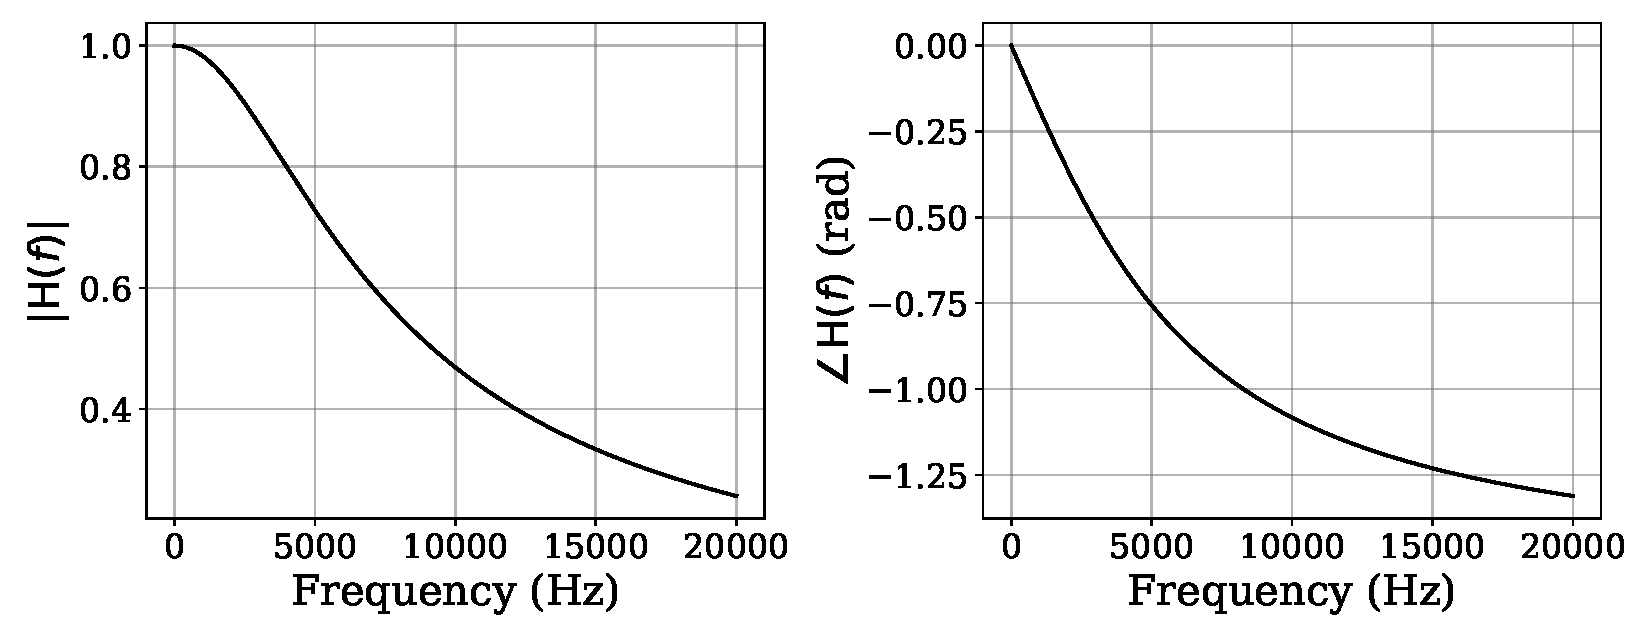
\includegraphics[width=\linewidth]{fig/LowPassFilterResponse.pdf}
				\end{figure}
		\end{enumerate}
	\end{frame}
	
	\begin{frame}{RC Circuit}
		\begin{enumerate}
			\item Taking $f = 5 \text{ kHz}$, we can predict the output by finding the correct points on the magnitude and phase plots:
				\begin{figure}
					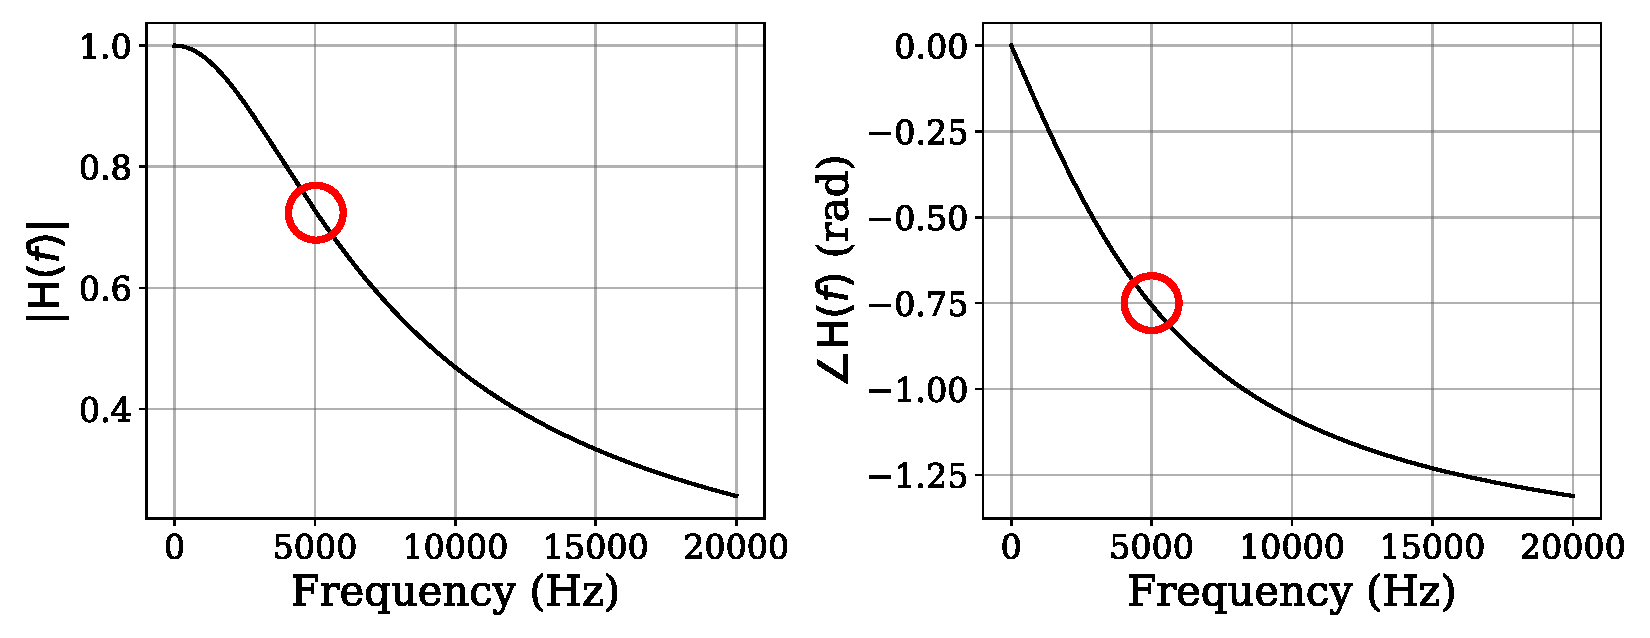
\includegraphics[width=\linewidth]{fig/LowPassFilterResponse_5kHz.pdf}
				\end{figure}
			\item We predict roughly:
				\begin{equation}
					y(t) = 0.7 \cdot \cos(2\pi f t - 0.75)
				\end{equation}
		\end{enumerate}
	\end{frame}
	
	\begin{frame}{RC Circuit}
		\begin{enumerate}
			\item Plotting the input and predicted output together, we get:
				\begin{figure}
					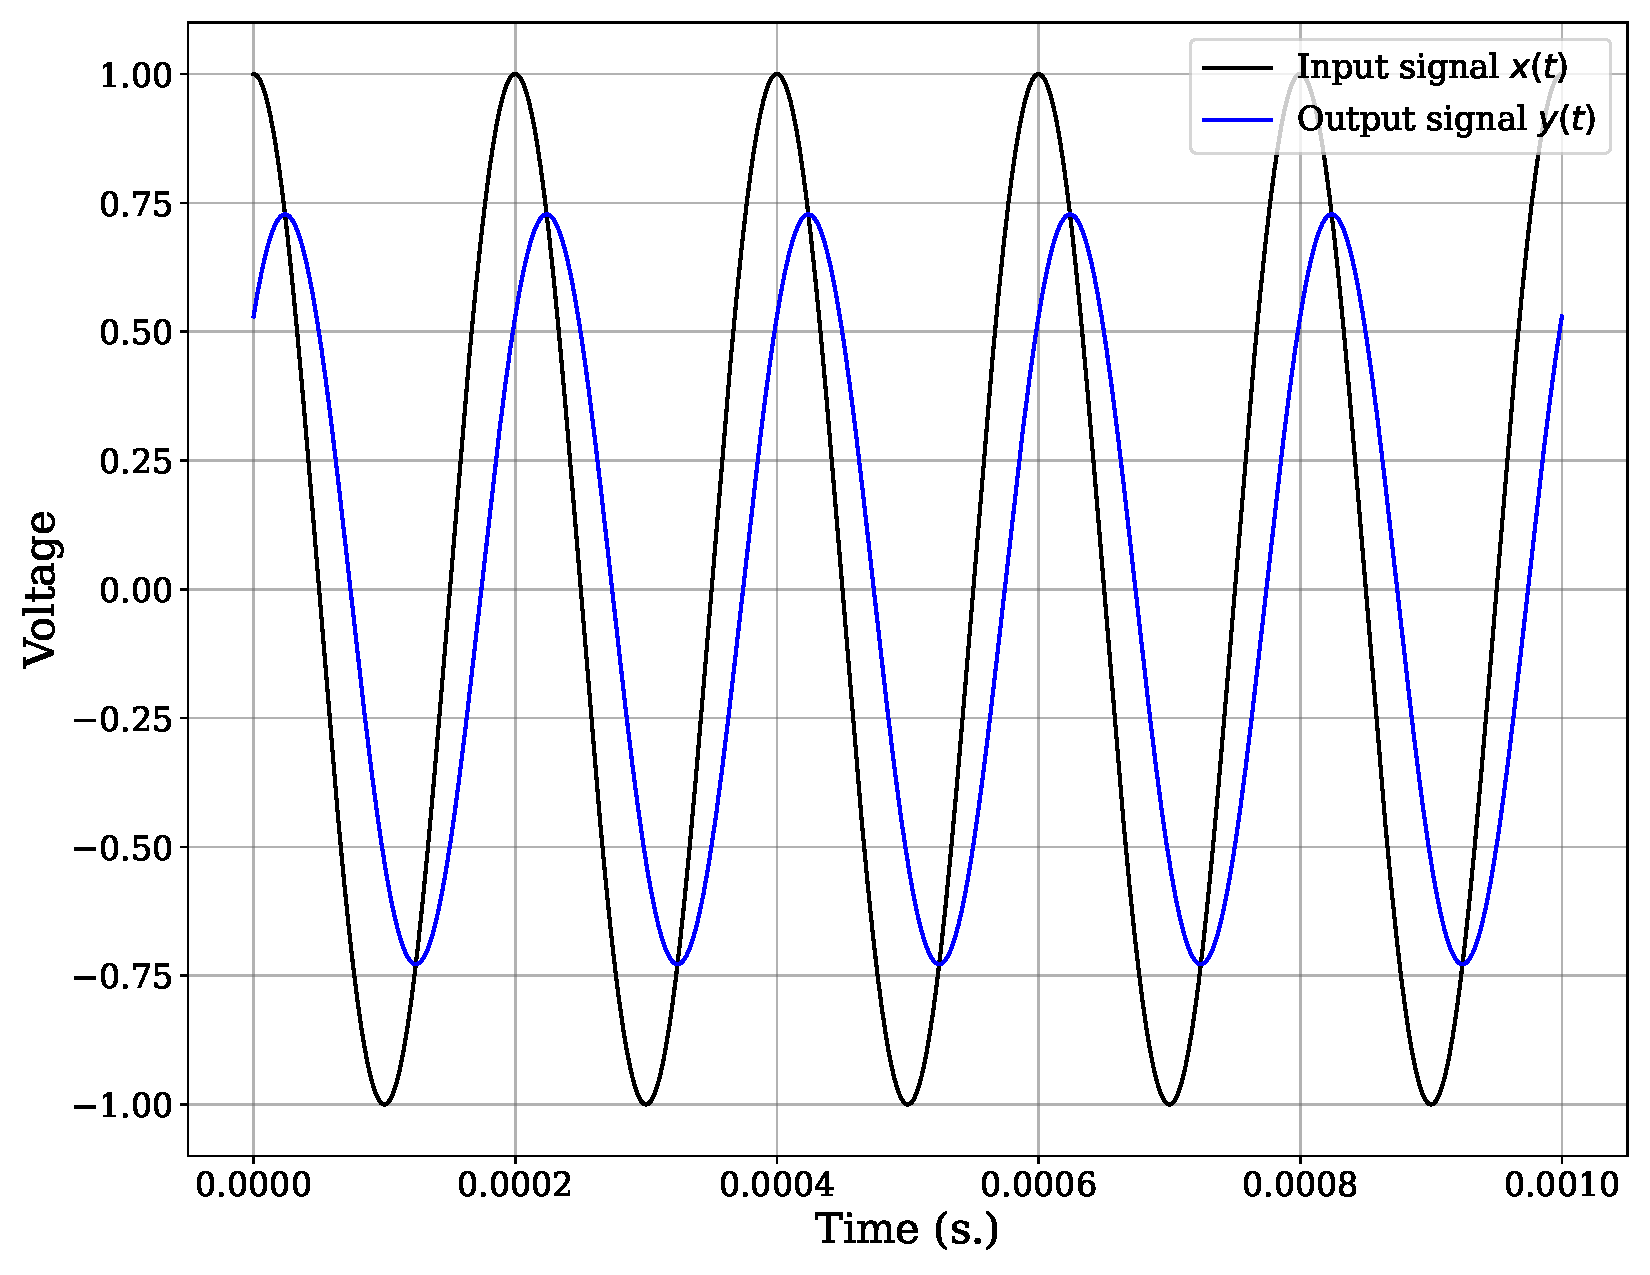
\includegraphics[width=0.65\linewidth]{fig/LowPassIO_5kHz.pdf}
				\end{figure}
			\item Let's compare this to a real circuit!
		\end{enumerate}
	\end{frame}
	
	\begin{frame}{RC Circuit}
		attach pictures from the demonstration here
	\end{frame}
	
	\begin{frame}{RC Circuit}
		\begin{enumerate}
			\item Now, let's try a slightly more complicated function to really test the bold statement of eqn. (\ref{eqn:output_to_arbitrary}) above.
			\item Consider the square wave signal plotted below:
				\begin{figure}
					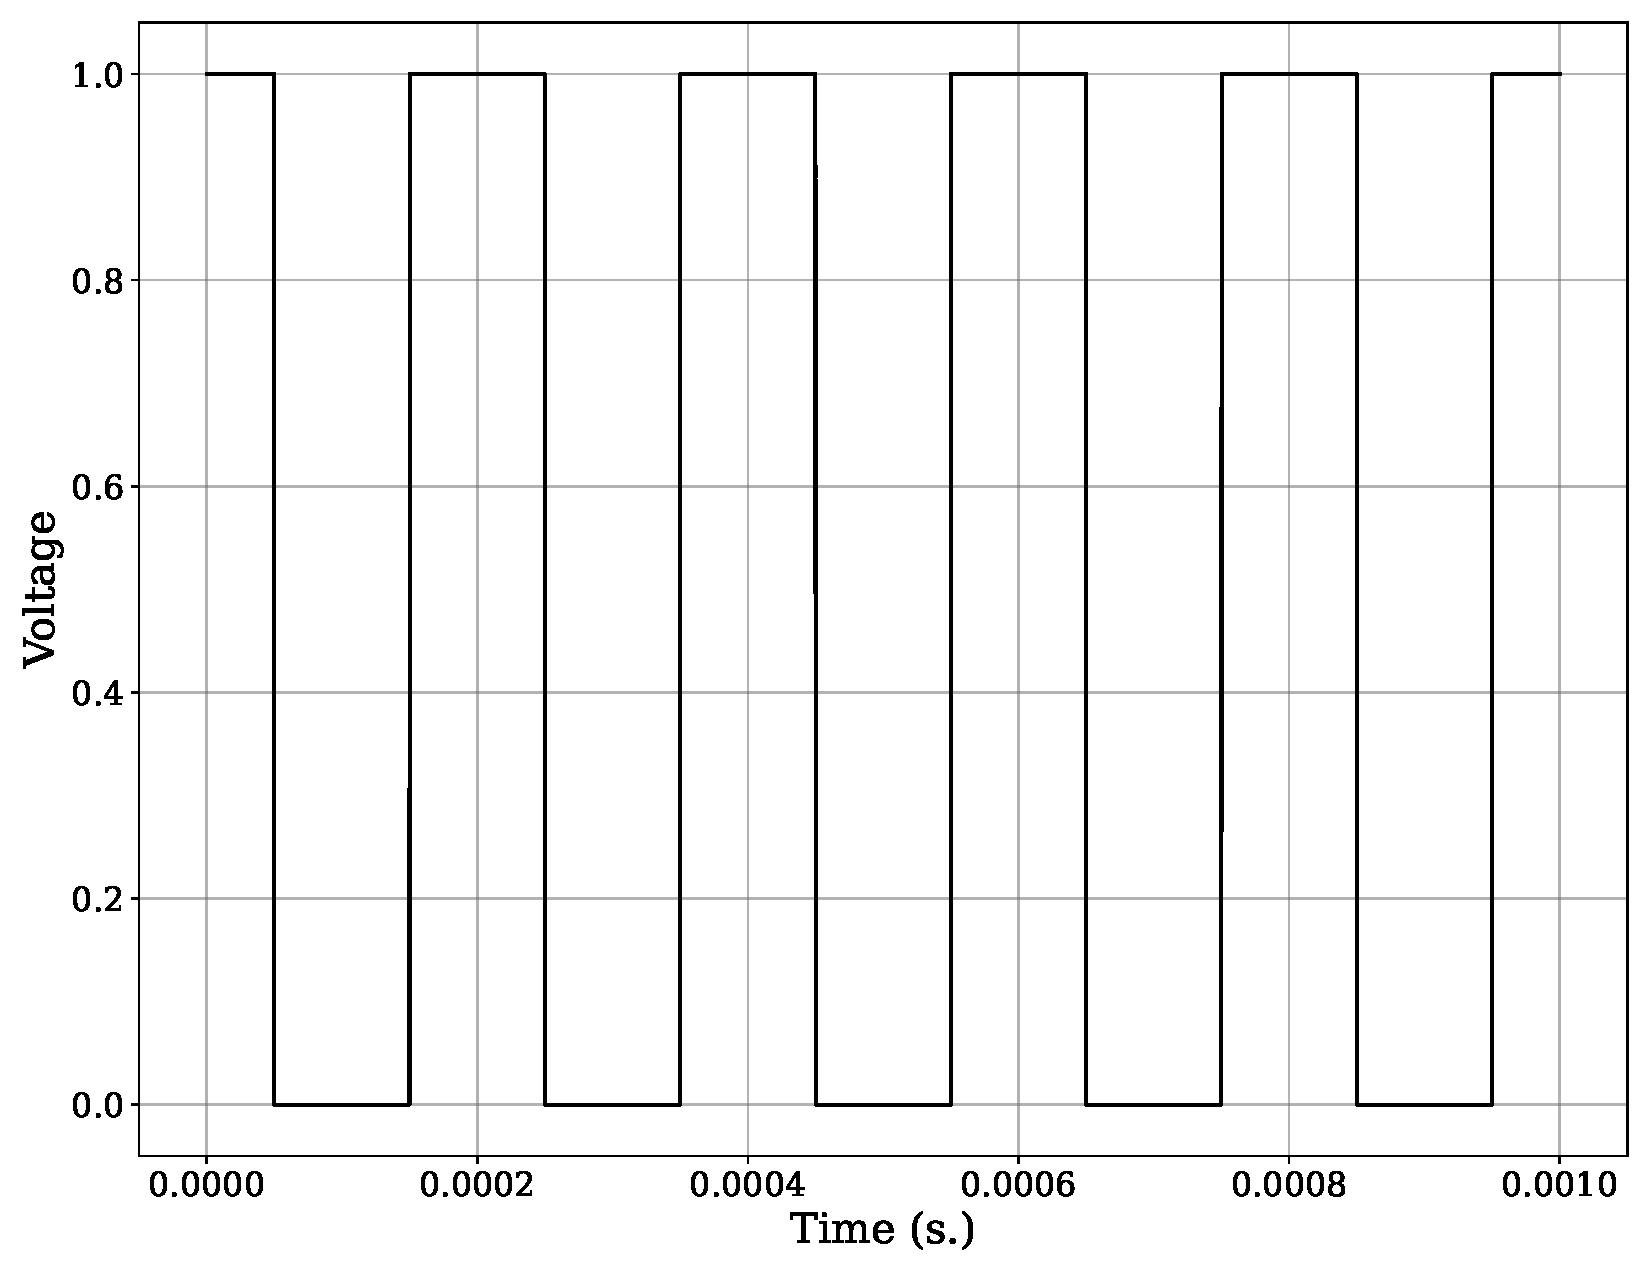
\includegraphics[width=0.65\linewidth]{fig/SquareWaveSignal.pdf}
				\end{figure}
		\end{enumerate}
	\end{frame}
	
	\begin{frame}{RC Circuit}
		\begin{enumerate}
			\item We will soon see that this signal can be represented as the following summation of sinusoids:
				\begin{equation}
					s(t) = \frac{1}{2} + 2 \sum_{n = 0}^{\infty} \left[\frac{2 \sin (n \pi / 2)}{n\pi}\right] \cos (2 \pi f n t)
				\end{equation}
			
			\item Using equation (\ref{eqn:output_to_arbitrary}) and (\ref{eqn:output_to_sinusoid}) above, we can predict the output:
				\begin{align} \label{eqn:rc_square_predicted_output}
					y(t) = &\frac{|H(0)|}{2}\cos(\angle H(0)) \\ &+ 2 \sum_{n = 0}^{\infty} H(2\pi f n t) \left[\frac{2 \sin (n \pi / 2)}{n\pi}\right] \cos (2 \pi f n t + \angle H(2\pi f n t))
				\end{align}	
		\end{enumerate}
	\end{frame}
	
	\begin{frame}{RC Circuit}
		\begin{enumerate}
			\item Using eqn. (\ref{eqn:rc_square_predicted_output}) and some python code, we predict the output of the circuit to be:
				\begin{figure}
					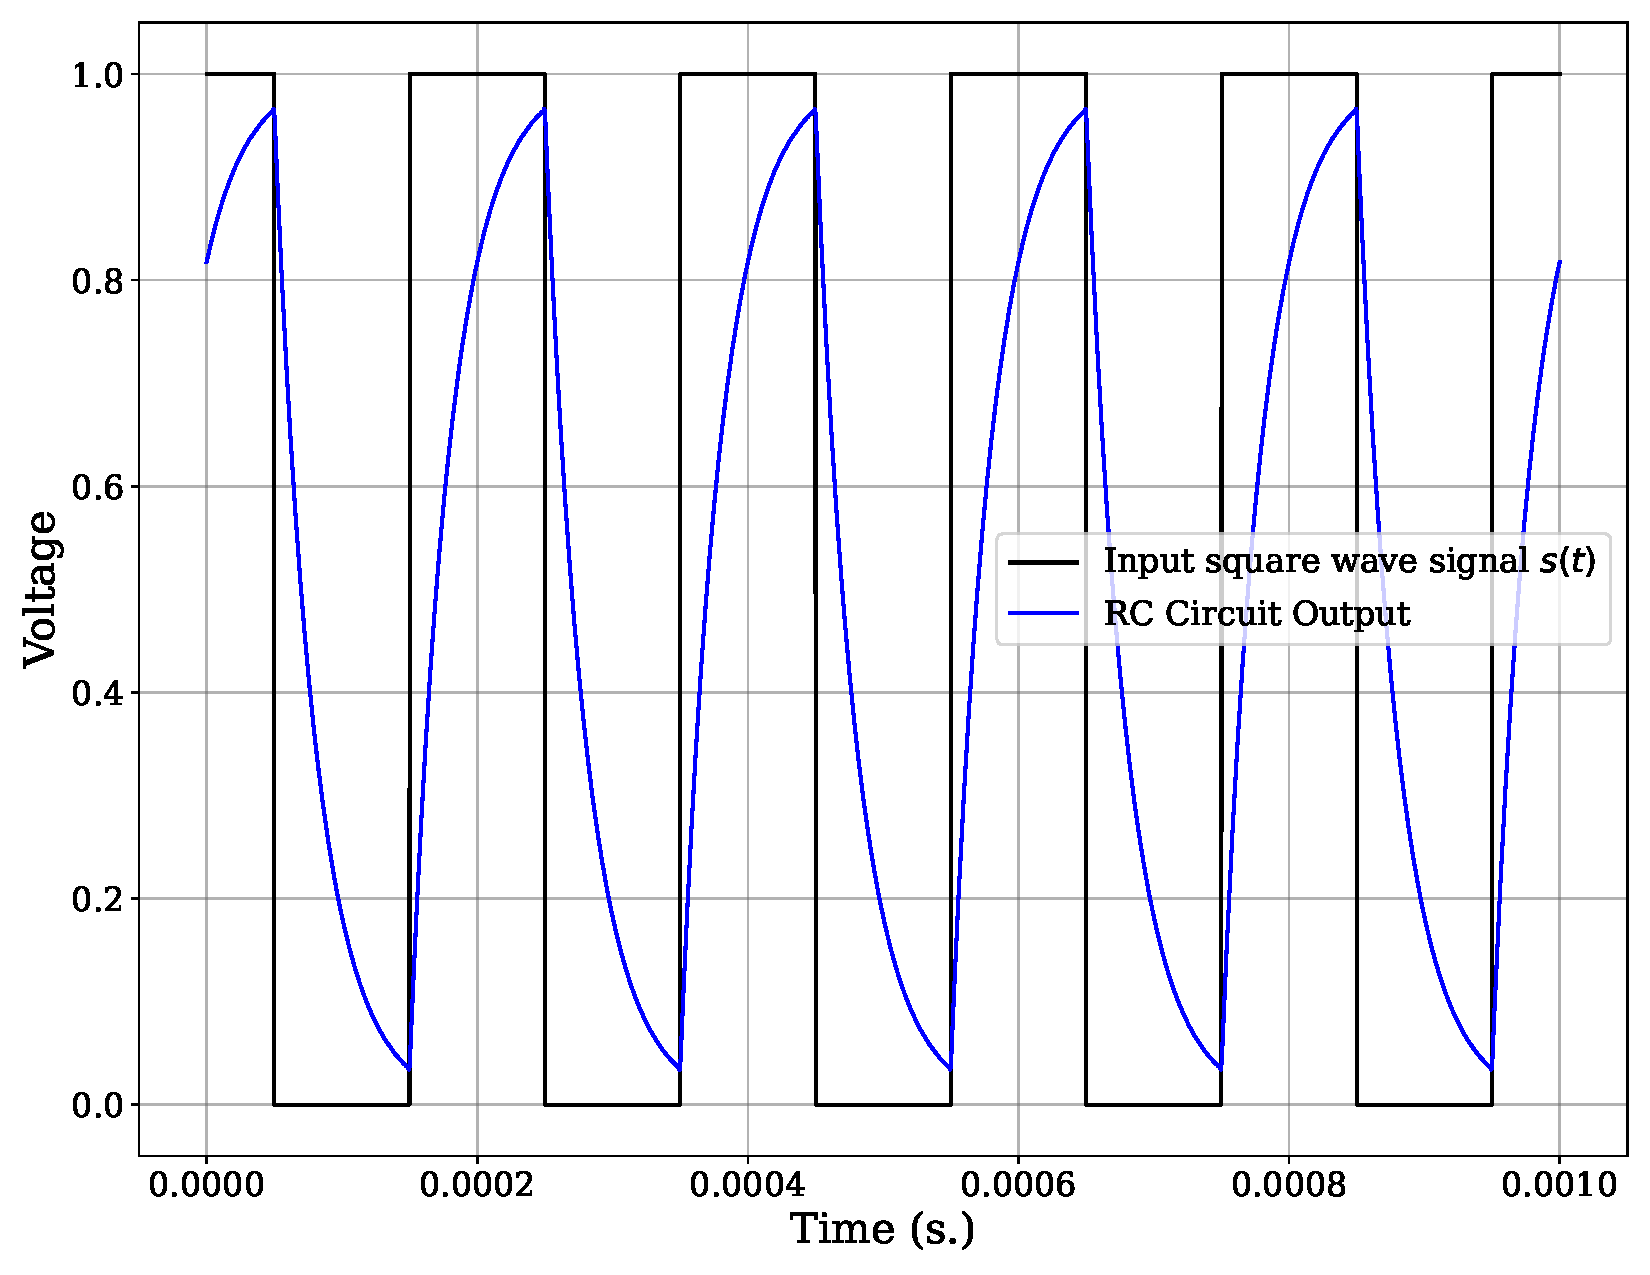
\includegraphics[width=0.65\linewidth]{fig/LowPassIO_Square.pdf}
				\end{figure}
			\item Of course, we need to check this with an actual circuit!
		\end{enumerate}
	\end{frame}
	
	\begin{frame}{RC Circuit}
		add pictures from the demonstration here
	\end{frame}
	
	\begin{frame}{RC Circuit: Summary}
		\begin{enumerate}
			\item In this lecture we analyzed an RC low-pass filter circuit. We saw that the output of the circuit to a sinusoidal input is just a scaled and phase shifted version of the input.
			\item We extended this result to say that if the input to the circuit is any summation of sinusoids, the output will be scaled and phase shifted versions of these same sinusoids.
			\item We checked both of these results by predicting the output of the filter to a single sinusoid and to a square wave and we verified that our predictions match the behavior of the real circuit.
			\item Fourier analysis consists of treating all input signals as summations of sinusoids and designing circuits and systems to manipulate these sinusoids in a desired manner.  
		\end{enumerate}
	\end{frame}
	
\end{document}